\documentclass[twocolumn]{article}
%\documentclass{ctexart}
\usepackage{multicol}
\usepackage{wrapfig}
\usepackage{lipsum}
%for long table
\makeatletter
\newenvironment{tablehere}
  {\def\@captype{table}}
 {}

\newenvironment{figurehere}
 {\def\@captype{figure}}
 {}
\makeatother
\usepackage{longtable}
%\documentclass{ctexart}
\usepackage{ctex}%中文
\usepackage{graphicx}
\usepackage{zhlipsum}
\usepackage{multirow}
\usepackage{biblatex}%biber才可以
\addbibresource{kgref.bib}
\usepackage{cuted}
%\graphicspath{{picture/}}
\usepackage[left=2.5cm,right=1.97cm,top=2.5cm,bottom=2.5cm]{geometry}%设置页边距
\renewcommand{\baselinestretch}{1.25}%行间距
%\usepackage[hidelinks,urlcolor=black,linkcolor=black]{hyperref}%引入超链接包,否则会出现Undefined sequence
\usepackage[hidelinks]{hyperref}
%[colorlinks,urlcolor=black,linkcolor=black]去除超链接中的颜色框
\usepackage{amssymb}%数学符号
\usepackage{amsmath}%数学公式
\usepackage{booktabs}%设置三线表的线粗细
\usepackage{array}%table
\newcommand{\tabincell}[2]{\begin{tabular}{@{}#1@{}}#2\end{tabular}}
%\usepackage{cite}
% \ctexset{section={format={\zihao{3} \heiti \bfseries}},
% bibname={\zihao{-4} \heiti \bfseries 参考文献}}

\newcommand{\upcite}[1]{\textsuperscript{\textsuperscript{\cite{#1}}}}
\usepackage{caption}
\DeclareCaptionFont{heiti}{\heiti}
\captionsetup{labelsep=quad,font={small,bf,heiti},skip={4pt}}
\usepackage{geometry}
%\title{\heiti \zihao{2} 融合}%黑体2号 在标题那页插入脚注

\author{\zihao{-4} \songti xxx}
\date{}
%%%%%%%%%%%%%%%%%%%%%%%%%%%%%%%%%%%%%%%
\begin{document}
	\section{融合多源信息}
	多源信息能够帮助构建更加精准的知识表示,
	经典的知识表示学习模型往往仅关注知识图谱自身固有的结构信息而忽略了蕴含在多源信息中的丰富知识。
	这些多源信息包括:类型信息,实体描述信息以及关系路径等,本章中将讨论如何将
	外部信息源融合进知识表示空间中学习以增强知识图谱中知识的表示。
	\begin{equation}
		L=\sum_{(h,r,t)\in \mathcal{S}}\sum_{(h',r,t')\in \mathcal{S}'}\max (0,f(h,r,t)+\gamma-f(h'+r-t'))
	\end{equation}
	\subsection{类别信息}
	最常用的类别信息就是实体类别,Guo等人\upcite{SSE}提出语义平滑嵌入模型(Semantically Smooth Embedding,SSE),基于的思想是属于同一语义类型的实体在嵌入空间中距离比较近。SSE利用两种流行学算法Laplacian eigenmaps和Locally linear embedding来约束这种平滑性假设。Lacian eigenmaps算法要求一个实体与它具有同类别的实体在嵌入空间中距离更近,这种约束形式用公式表示为:
	\begin{equation}
		\mathcal{R}_1 =\left \| \textbf{h}-\textbf{t} \right \|_2^2w_{ht}^{(1)}
	\end{equation}
	其中$\textbf{h},\textbf{t}$分别是实体$h,t$的嵌入表示,$w_{ht}^{(1)}$代表两个实体之间的邻接矩阵,当两个实体$h$和$t$属于同一类型时,$w_{ht}^{(1)}=1$,反之为0。
	Locally linear embedding算法要求一个实体可以由它临近的实体经过线性组合表示出来。这里临近的实体就是指属于同一个类别的实体,这种约束形式用公式表示为:
	\begin{equation}
	\mathcal{R}_2=\left \| \textbf{h}-\sum _{t\in \mathbb{N}(h))}w_{ht}^{(2)}\textbf{t} \right \|_2^2
	\end{equation}
	其中$\mathbb{N}(h)$代表与实体$h$类型相同的$K$个实体集合,集合的个数$K$是一个超参数。
	当实体$t$在集合$\mathbb{N}(h)$中,则$w_{ht}^{(2)}$为1,反之为0。
	SSE模型的能量函数与TransE\upcite{TransE}模型一致,
	将$\mathcal{R}_1$,$\mathcal{R}_2$加到最大间隔方法里作为整个模型损失函数的一个正则化项从而达到约束嵌入空间语义平滑的作用。实验表明,SSE模型学习后的嵌入空间中,语义类别一致的实体很好的聚在了一起。
	
	SSE模型的缺点在于默认所有实体只有一个类别,而现实世界中的实体不仅有多个类别而且每一个类别是有层次结构的。如图1所示,
	\begin{figure}[ht]
		\centering
		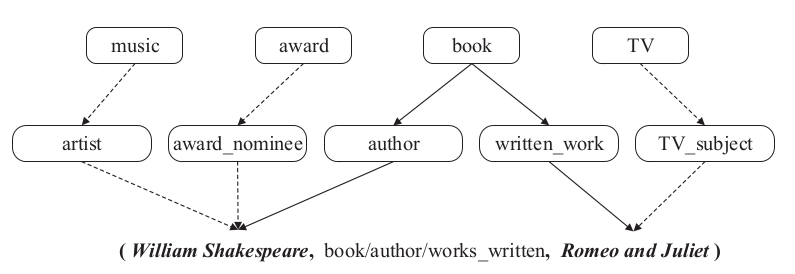
\includegraphics[width=\linewidth]{TKRL.png}
		\caption{取自TKRL\upcite{TKRL}}
	\end{figure}
	从图中可以看到头实体William Shakespeare存在很多实体类型,而且每一个实体类型都有子类型。
	基于以上问题,Xie等人\upcite{TKRL}提出一种融合实体层次类型信息的模型TKRL(type-embodied knowledge representation learning),引入具有层次结构的实体类别信息以及与关系之间的约束信息,
	TKRL模型的能量函数定义为:
	\begin{equation}
		f(h,r,t)=\left \| M_{r,h}h+r-M_{rt}t \right \|
	\end{equation}
	其中$M_{r,h},M_{r,t}$分别表示的是头实体和尾实体的层次类型映射矩阵,
%	是指头实体和尾实体在关系$r$下应该凸显哪一个类型。如图1中的例子头实体William Shakespeare在book/author/works\_written关系下应该凸显book/author实体类型。
%	为了达到这个目的,
	由于一个类别有多个子类别,TKRL为每一个子类型也设置了映射矩阵,使用这些子类型的映射矩阵构建层次类型映射矩阵。
	以头实体$h$为例,$h$类别集合是$c=\{c_1,c_2,\cdots,c_n\}$,$n$代表类别数目,$c_i$是$h$的第$i$个类别,每一个类别有很多个子类别,$c_i=\{c_i^1,c_i^2,\cdots,c_i^m\}$,$m$代表类别$i$的子类别的个数,其中$c_i^j$代表$h$的第$i$个类别的第$j$个子类别。头实体$h$的类型映射矩阵表示为:
	\begin{equation}
		M_{rh}=\alpha_1 M_{c_1^h}+\alpha_2 M_{c_2^h}+\cdots+\alpha_n M_{c_n^h}
	\end{equation}
	其中$M_{c_i^h}$代表$h$在它的第$i$个类型下的映射矩阵,$\alpha_i$就是权重,表示的就是$h$在当前第$i$个类别下的凸显程度,尾实体$h$的类型映射矩阵计算方式同理。
	为了进一步的处理层次类型信息,TKRL采用两种层次编码器。第一种是递归层次编码器:
	\begin{equation}
		M_{c_i^h}=\prod_{j=1}^{m}M_{c_i^h}^{(j)}=M_{c_i^h}^{(1)}M_{c_i^h}^{(2)}\cdots M_{c_i^h}^{(m)}
	\end{equation}
	第二种是加权层次编码器:
	\begin{equation}
		\begin{split}
		M_{c_i^h}=&\sum_{j=1}^{m}\beta_jM_{c_i^h}^{(j)}\\
		=&\beta_1M_{c_i^h}^{(1)}+\beta_2M_{c_i^h}^{(2)}+\cdots+\beta_mM_{c_i^h}^{(m)}
		\end{split}
	\end{equation}
	其中$M_{c_i^h}^{(j)}$代表的是头实体$h$的第$i$个类型的第$j$个子类型的映射矩阵。TRKL的损失函数采用做大间隔方法。
	
	\noindent 实体类别信息还能在模型中作为类别限制,帮助模型学习更好的知识表示。不同于Krompaß等人\upcite{typeconstrain}使用硬类型限制控制负例三元组的生成,强制替换的实体与原来的实体具有同样的类别,TKRL模型采用一种软类型限制(Soft Type Contraint,STC)机制,STC的策略是以某一定的比例选取那些与被替换实体有相同类型的实体,如下公式
	\begin{equation}
		P(\widetilde{e}\in E_c)=\frac{(k+1)\left | E_c \right |}{\left | E \right |+k\left | E_c \right |}
	\end{equation}
	其中$E$是三元组集合,$E_c\in E$代表的一个实体集合其中所有实体都有类别$c$,$k$是一个超参数。
	%含义是选取在$E_c$集合中的实体作为负例三元组的几率是选取那些不在$E_c$集合中的实体几率的$k$倍。
	
	在测试时对于给定的一种关系,TKRL模型限定这种关系的头尾实体的具体类别,这种做法泛化型不高并且并不是所有的实体都具有层次类别。针对这些问题,Jin等人\upcite{TEKRL}提出的TEKRL模型解决了其它模型在引入实体类别信息时额外添加规则的问题,TEKRL直接利用数据集中最底层的实体类别,通过引入注意力机制学习实体类别与关系之间的相关性,通过对实体类别表示加权求和取代制定实体类别和关系之间约束的操作。
	TEKRL模型为每一个实体构建基于结构和基于类别的两种实体表示,模型的能量函数定义为:
	\begin{equation}
		f=f_{ss}+\beta f_{cc} \notag
	\end{equation}
	其中$\beta$用来调整基于类别的表示在模型中的作用大小,$f_{ss}$和$f_{cc}$分别代表基于结构的能量函数和基于类别的能量函数。
	\begin{gather}
		f_{ss}=\left \| \textbf{h}_s+\textbf{r}-\textbf{t}_s \right \| \notag \\
		f_{cc}=\left \| \textbf{h}_c+\textbf{r}-\textbf{t}_c \right \| \notag 
	\end{gather}
	$\textbf{h}_s$和$\textbf{t}_s$是基于结构的实体表示,它们通过知识图谱中结构化信息学习。$\textbf{h}_c$和$\textbf{t}_c$是基于类别的实体表示,通过注意力机制得到实体类别表示与三元组中关系的相关性,然后对所有类别的表示加权求和作为实体的基于类别的表示。
	
	除了考虑实体类别信息外,Zhang等人\upcite{HRS}提出一种利用关系层次结构的知识表示模型HRS(Hierarchical Relation Structure)。HRS将知识图谱中的关系划分为一个三层的层次结构,顶层关系$r_c$是由语义相近的关系聚类而成,中间层指特定的关系$r'$,底层关系$r_s$是将每一个关系再进一步的划分成多个子关系。
	在训练时,对于每一个三元组$(h,r,t)$,其中关系$r$的嵌入表示$\textbf{r}$为三层关系的嵌入表示之和
	$\textbf{r}=\textbf{r}_c+\textbf{r}'+\textbf{r}_s$。
	HRS模型的损失函数定义为
	\begin{equation}
		L=L_{Orig}+L_{HRS}
	\end{equation}
	其中$L_{Orig}$采用经典模型TransE,TransR等的最大间隔方法,$L_{HRS}$作为正则化项约束模型学习层次关系的表示。
	\begin{equation}
		L_{HRS}=\lambda_1\sum_{\textbf{r}_c\in \mathcal{C}}\left \| \textbf{r}_c \right \|_2^2+\lambda_2\sum_{\textbf{r}'\in \mathcal{R}}\left \| \textbf{r}' \right \|_2^2+\lambda_3\sum_{\textbf{r}_s\in\mathcal{S}}\left \| \textbf{r}_s \right \|_2^2
	\end{equation}
	其中$\mathcal{C}$,$\mathcal{R}$,$\mathcal{S}$分别代表关系聚类集合,关系集合,子关系聚类集合。
	此外在知识图谱中某些关系代表的是实体的属性信息,而属性与关系的区别在于属性有明显的一对多关系。Lin等人\upcite{EAR}提出一种知识表示模型从所有的关系分离出关系与属性,然后再建模实体表示、关系表示、属性表示。
	
	
\subsection{文本描述}
	知识图谱中很多实体都是带有描述信息的,这些信息能够作为知识图谱中结构化信息的辅助,帮助模型学习更精准的知识表示,知识库的构建资源也往往是从文本中获取,因此实体描述文本能天然的与知识空间进行交互。
	如图2所示。
	\begin{figure}[ht]
		\centering
		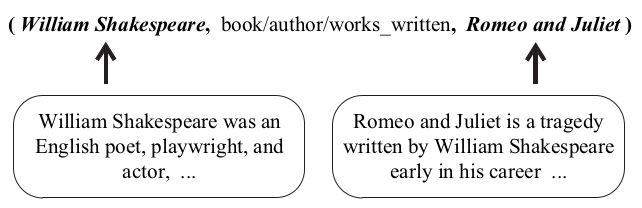
\includegraphics[width=0.8\linewidth]{dkrl.png}
		\caption{取自DKRL\upcite{DKRL}}
\end{figure}
	这些描述文本是对实体相关信息的详细描述。
%	这些文本可以认为是对知识图谱中结构化信息的补充,利用这些实体的文本信息有助于建模知识图谱的语义关系从而得到更加精准的知识表示。
	那些仅仅基于知识图谱结构化信息的知识表示模型无法处理不在知识图谱中的实体(out of KG),而联合文本嵌入的方式可以做到互补使得模型学习到那些在文本中出现而不在知识图谱中的实体。
	
	Wang等人\upcite{Wang}首先提出联合知识图谱和实体描述文本的知识表示学习模型,模型基于TransE\upcite{TransE}和Skip-gram\cite{Skipgram}模型的思想。整个模型分成三个部分:知识模型、文本模型、对齐模型。
	知识模型基于平移模型的思想学习实体和关系的表示,损失函数定义如下:
	\begin{equation}
	\begin{split}
	\mathcal{L}_K=-&\sum_{(h,r,t)}\log \text{Pr}(h|r,t) \\
	+& \log \text{Pr}(t|h,r)+\log \text{Pr}(r|h,t)
	\end{split}
	\end{equation}
	%知识模型用来学习知识图谱中三元组的表示,
	以\text{Pr}(h|r,t)为例:
	\begin{gather}	
	\text{Pr}(h|r,t)=\frac{\exp{z(h,r,t)}}{\sum_{\widetilde{h}}\exp{z(\widetilde{h},r,t)}} \\
	z(h,r,t)=b-\frac{1}{2}\left \| \textbf{h}+\textbf{r}-\textbf{t} \right \|_2^2
	\end{gather}
	
	文本模型用来学习实体描述文本中单词的表示,基于Skip-gram的思想,定义文本模型的损失函数如下:
	\begin{equation}
	\mathcal{L}_T=-\sum_{(w,v)\in \mathcal{C}}\log \text{Pr}(w|v)
	\end{equation}
	其中$\text{Pr}(w|v)$代表两个单词在滑动窗口内的共现概率,$\mathcal{C}$代表滑动窗口内共现单词的集合。
	\begin{gather}
	\text{Pr}(w|v)=\frac{\exp{z(w,v)}}{\sum_{\widetilde{w}}\exp{z(\widetilde{w},v)}} \\
	z(w,v)=b-\frac{1}{2}\left \|\textbf{w}-\textbf{v}  \right \|_2^2
	\end{gather}

%	文本模型利用Skip-gram模型的思想学习文本中单词的词向量,
	最后对齐模型实现知识空间和文本空间对齐,对齐原则是利用实体名称或者维基百科锚文本。模型的损失函数为这三个子模块之和
	\begin{equation}
	\mathcal{L}=\mathcal{L}_K+\mathcal{L}_T+\mathcal{L}_A
	\end{equation}
%	其中$\mathcal{L}_K$,$\mathcal{L}_T$,
	$\mathcal{L}_A$是对齐模型的损失函数。
	但是由于实体名称歧义性较大的问题利用实体名称对齐的原则会打乱文本原有的语义空间,
%	\begin{equation}
%		\mathcal{L}_A=\sum_{(w,v)\in \mathcal{C},v\in \mathcal{A}}\log \text{Pr}(w|e_v)
%	\end{equation}
%	其中$\mathcal{A}$表示锚文本的集合,$e_v$代表实体描述文本中单词$v$所对应的在锚文本中的实体。
	而利用维基百科锚文本对齐的原则依赖于特定的数据源,这使得这种方式无法应用到其它数据源领域。
	为了解决以上问题,Zhong等人\upcite{Zhong}提出利用实体描述文本作为对齐原则,定义对齐模块的损失函数为:
	%在以上的知识表示学习模型的基础上做了改进。在对齐模型的损失函数$\mathcal{L}_A$,利用实体描述文本作为对齐原则,认为实体的表示向量应当与描述文本单词的词向量尽可能接近。
	
	\begin{equation}
		\mathcal{L}_A=-\sum_{e\in E}\sum_{w\in D_e}\log \text{Pr}(w|e)+\log \text{Pr}(e|w)
	\end{equation}
	$E$代表知识图谱中的实体集合,$D_e$代表实体$e$的描述文本,\text{Pr}(w|e)和\text{Pr}(e|w)的计算方式见公式(15),(16)。类似的还有Zhang等人\upcite{JointS}也尝试使用实体名称和实体描述文本中词向量的均值作为实体的文本表示。
	
	以上的模型考虑的是单词级别的文本信息而没有利用整个文本的语序语义信息。Xie等人\upcite{DKRL}
	提出一种融合实体描述的知识表示模型(Description-embodied knowledge representation learning,DKRL)。DKRL在TransE模型的基础上融合实体描述的文本信息,为每一个实体设置两种知识表示。第一种是基于知识图谱结构化信息的表示,可以随机初始化或者利用TransE模型预训练好的实体表示。
	第二种是基于文本描述的表示,使用连续词袋(continuous bag-of-words,CBOW)模型和卷积神经网络(Convolutional neural network,CNN)模型从文本中构建。给定三元组$(h,r,t)$,DKRL模型的能量函数定义如公式:
	\begin{equation}
		\begin{split}
			E(h,r,t)=&||\textbf{h}_S+\textbf{r}-\textbf{t}_S||+||\textbf{h}_S+\textbf{r}-\textbf{t}_D|| \\ 
			+&||\textbf{h}_D+\textbf{r}-\textbf{t}_S||+||\textbf{h}_D+\textbf{r}-\textbf{t}_D||
		\end{split}
	\end{equation}
	其中$\textbf{h}_S/\textbf{h}_D$,$\textbf{t}_S/\textbf{t}_D$分别代表头实体/尾实体的基于结构的表示和基于实体描述的表示,$\textbf{r}$代表关系的知识表示。通过混合项$||\textbf{h}_S+\textbf{r}-\textbf{t}_D||$,
	$||\textbf{h}_D+\textbf{r}-\textbf{t}_S||$的限制,DKRL模型将实体的两种不同的表示向量映射到同一个语义空间中。实验结果表明DKRL模型在很多知识图谱任务上效果表现很好。
	然而DKRL模型是一种弱关联建模,在融合实体基于结构的表示和基于文本的表示时没有足够的交互过程。
	Xiao等人\upcite{SSP}提出语义空间投影模型(Semantic space projection,SSP),将三元组的嵌入表示投影到语义子空间上,在语义子空间上学习实体的两种表示。与DKRL不同的是SSP采用主题(topic)模型建模实体的文本表示。
	
	Wang等人\upcite{TEKE}提出一种增强型文本知识嵌入模型(Text-enhanced knowledge embedding,TEKE)。TEKE不仅将文本信息融入到知识图谱的空间中,并且每一个关系对于不同的头实体和尾实体都有不同的表示,这样可以更好的解决1-N,N-1以及N-N的关系问题。首先使用实体连接工具标注出文本中是知识图谱中实体的单词并且基于这些实体单词构建共现网络(co-occurrence network)。
%	设为$\mathcal{G}=(\mathcal{X,Y})$
%	定义$x_i\in \mathcal{X}$,其中$x_i$代表网络的节点,它就是实体单词。$y_{ij}\in \mathcal{Y}$代表两个实体单词共同出现的频次。
	对于文本中的实体单词$e$,定义它的上下文集合为$n(e)$,它的文本向量表示为$\textbf{n}(e)$,$\textbf{n}(e)$是$n(e)$中所有单词词向量的加权求和,权重为两个实体单词共同出现的频次归一化后的值。给定三元组$(h,t,r)$,TEKE模型认为两个实体$h,t$的上下文集合$n(h)$,$n(t)$中共同出现的单词往往反映着两个实体之间的关系,
	定义$n(h,t)=n(h)\cap n(t)$作为两个实体上下文的匹配集合,其向量表示为$\textbf{n}(h,t)$。
%	它是$n(h,t)$中所有实体匹配表示的加权求和,可以看出当$h$或$t$不同时关系的表示也是不同的,因此TEKE模型可以很好的处理1-to-N,N-to-1,N-to-N关系。
	最后将文本的语义空间映射到知识图谱的语义空间:
	\begin{gather}
		\widehat{h}=\textbf{n}(h)A+\textbf{h} \notag \\
		\widehat{r}=\textbf{n}(h,t)B+\textbf{r} \\
		\widehat{t}=\textbf{n}(t)A+\textbf{t} \notag
	\end{gather}
	其中$A,B$是映射矩阵,$\textbf{h},\textbf{r},\textbf{t}$是偏置项,它们都是可学习的参数,
	%词向量利用Word2Vec工具预训练。
	模型的能量函数定义为$f(h,r,t)=\left \|\widehat{h}+\widehat{r}-\widehat{t}\right \|_2^2$,利用最大间隔方法训练。
	
	然而TEKE模型并没有考虑到实体和关系的模糊性,所谓模糊性是指关系所表达的精确语义依靠于头尾实体的语义。此外两个实体单词的上下文集合中共同出现的单词并不能总是表达两个实体单词之间的关系,这种方式会给某些三元组带来噪声信息。基于以上问题,An等人\upcite{ATEKE}提出ATEKE模型,利用实体描述文本和特定三元组的关系提及(relation mention)来增强实体和关系的表示。为了处理噪声的问题,在提取关系提及时添加两个约束条件:(1)包含特定三元组的两个实体以及关系的下义词或同义词;(2)关系和句子中某一单词的相似性超过阈值。满足两个约束条件之一的句子被认为是准确的关系提及。通过注意力机制计算关系提及和实体描述的相关性,得到
	三元组($h,r,t$)的文本表示($\textbf{h}_D,\textbf{r}_D,\textbf{t}_D$)。最后将基于文本的表示和基于结构的表示加权求和作为实体表示。
	\begin{gather}
		Re(\textbf{h})=\alpha Re(\textbf{h}_{S})+(1-\alpha)\textbf{h}_D \notag \\
		Re(\textbf{r})=\alpha Re(\textbf{r}_{S})+(1-\alpha)\textbf{r}_D \notag \\
		Re(\textbf{t})=\alpha Re(\textbf{t}_{S})+(1-\alpha)\textbf{t}_D \notag
	\end{gather}
	其中$0\leq \alpha \leq 1$,$Re$表示取向量的实值部分。
\subsection{关系路径}
关系路径是指两个实体之间的多步关系而不仅仅限于两个实体之间直接相连的关系。多步关系包含了两个实体之间丰富的语义关系,多步推理。

Lin等人\upcite{PTransE}提出PTransE模型,在TransE模型的基础上将两个实体之间的多步关系路径看做两个实体之间相连的关系。由于两个实体之间存在大量的关系路径,PTransE模型采用路径约束资源分配(path-constraint resource allocation,PCRA)算法提取出可以用来建模两个实体之间关系的可靠的关系路径。PTransE模型
的优化目标分为两部分:第一部分是利用TransE模型建模两个实体之间直接相连的关系;第二部分是建模两个实体之间多关系路径。
定义$P(h,t)=\{p_1,p_2,\cdots,p_N\}$代表实体$h$和$t$之间的多关系路径的集合,
模型的能量函数定义如下
\begin{equation}
	G(h,r,t)=f(h,r,t)+f(h,p,t)
\end{equation}
其中$f(h,r,t)$即为公式(1)中TransE模型的能量函数。
$p=(r_1,r_2,\cdots,r_l)$,它是给定头实体$h$和尾实体$t$下的某一条多步关系路径,$r_i$代表路径$p$上的第$i$个关系,$l$是路径上关系的个数。
%\begin{equation}
%	E(h,P,t)=\frac{1}{Z}\sum_{p\in P(h,t)}R(p|h,t)E(h,p,t)
%\end{equation}
%其中$R(p|h,t)$代表给定实体$h$和$t$的条件下多跳关系路径$p$的可靠性。$Z$为归一化因子,它是$h$和$t$的所有多跳关系路径的可靠性之和。
$f(h,p,t)$代表给定实体$h$和$t$以及多跳关系路径$p$的能量函数。
\begin{equation}
	f(h,p,t)=\left \| \textbf{p}-\textbf{r} \right \|
\end{equation}
$\textbf{p}$代表关系路径$p$的向量表示。PTransE模型采用三种方式计算$\textbf{p}$。
\begin{gather}
	\textbf{p}=\textbf{r}_1+\textbf{r}_2+\cdots+\textbf{r}_l \quad \text{ADD}\notag \\
	\textbf{p}=\textbf{r}_1\cdot\textbf{r}_2\cdots\cdot\textbf{r}_l \quad \text{MUL}\notag \\
	\textbf{c}_i=f(W[\textbf{c}_{i-1};\textbf{r}_i]) \quad \text{RNN} \notag
\end{gather}
ADD表示将路径上所有关系的向量表示相加,MUL表示相乘,RNN代表利用循环神经网络,此时$\textbf{p}$为路径上最后一个关系的隐藏状态。
模型的目标函数为:
\begin{equation}
	L=L(h,r,t)+\frac{1}{Z}\sum_{p\in P(h,t)}R(p|h,t)L(h,p,t)
\end{equation}
$L(h,r,t)$为公式(1)中TransE模型的目标函数,$R(p|h,t)$是利用PCRA算法计算的给定头尾实体$h$,$t$下关系路径$p$的可信度,$Z$是规范化因子,$L(h,p,t)$用来建模实体基于关系路径的表示,能量函数为$f(h,p,t)$。
%\begin{equation}
%L(h,p,t)=\sum_{(h,r,t)\in \mathcal{S}}\sum_{(h',r,t')\in \mathcal{S}'}\max (0,f(h,p,t)+\gamma-f(h'+p-t'))
%\end{equation}

Guu等人\upcite{Guu}提出另一种融合多步关系路径的知识表示学习模型,利用关系路径构建新的三元组并且对TransE模型和RESCAL\upcite{RESCAL}模型进行了扩展。给定头实体$h$和尾实体$t$以及长度为$l$的多跳关系路径$p$,扩展TransE模型后能量函数为
\begin{equation}
	f(h,p,t)=\left \| \textbf{h}+\textbf{r}_1+\cdots+\textbf{r}_l-\textbf{t} \right \| \notag
\end{equation}
扩展RESCAL模型后的能量函数为:
\begin{equation}
	f(h,p,t)=\textbf{h}^T(\textbf{M}_1\circ\cdots\circ\textbf{M}_l)\textbf{t} \notag
\end{equation}
上面两个模型的共同点都是从众多关系路径中选择一部分子集同时限制路径的长度为2步或者3步,Toutanova等人\upcite{Toutanova}利用动态规划算法建模两个实体之间所有可能的关系路径。

两条头尾实体相同的多步关系路径,即使路径中间的关系也相同但是由于路径中间实体的不同,两条路径表达的也可能是不同的含义。基于这个问题
Seo等人\upcite{RKRL}提出RKRL模型,同时考虑关系路径上中间的实体和关系信息。
%给定三元组$(h,r,t)$以及$h$和$t$之间的某条多步关系路径$p=\{r_1,e_1,\cdots,r_{n-1},e_{n-1},r_n\}$。

其中$\textbf{r}_i$代表多步关系路径上第$i$个关系的表示。
RKRL模型的能量函数和损失函数与PTransE模型一致,见公式(21),(23)。其中基于关系路径的能量函数定义为:
\begin{gather}
f(h,p,t)=\left \|\textbf{h}+\textbf{p}-\textbf{t} \right \| \notag \\
\textbf{p}=W_{e_1}\textbf{r}_1+\cdots+W_{e_{l-1}}\textbf{r}_{l-1}+\textbf{r}_l \notag
\end{gather}
%\begin{gather}
%	G(h,r,t)=f(h,r,t)+f(h,P,t)  \notag \\ 
%	f(h,P,t)=\frac{1}{Z}\sum_{p\in P}R(p|h,t)f(h,p,t) \notag
%\end{gather}
%其中$R(p|h,t)$代表给定实体$h$和$t$的条件下多跳关系路径$p$的可靠性,
%$Z$是规范化因子,它是$h$和$t$的所有多跳关系路径的可靠性之和。
RKRL采用两种特征来衡量路径$p$的可靠性,第一种特征是PTransE中提出的资源分配算法PCRA,但是由于该算法仅仅依靠资源流动的量来衡量可靠性可能不足以判别路径的语义关系,因此额外添加路径上与实体相连的关系出现的频率这一特征。


\subsection{其它信息}
除了可以融入上面三种信息源外,还有一些其它的信息也可以融入到知识图谱的语义空间中,增强知识的语义表示。
如Xie等人\upcite{IKRL}提出的IKRL模型,尝试融合实体图像信息学习实体跨模态的知识表示,与TKRL模型类似仍然是为每一个实体设置两种知识表示,基于结构的和基于图像的表示,采用AlexNet\upcite{Alexnet}网络作为图像的特征提取器,模型的能量函数和损失函数与TKRL一致。

以上介绍的知识表示学习模型都是将知识图谱看做三元组的集合,孤立的学习每个三元组的表示,尽管融合多步关系路径的模型引入了其它的实体和关系,但是绝大部分模型也只是将关系路径看做是两个实体之间的新关系,知识图谱的图结构信息并没有被完全利用。Feng等人\upcite{GAKE}提出一种图感知的表示学习模型GAKE(graph aware knowledge embedding),模型给出一个新的概念graph context。Graph context定义为知识图谱中与一个实体有关联的三种集合:neighbor context,path context和edge context。Neighbor context是一个实体的三元组集合
,path context是与一个实体相连的关系路径集合,edge context是一个实体所有的关系集合。由于不同的实体和关系对于一个实体的影响不同,GAKE利用注意力机制赋予不同关系和实体不同的权重。实验证明这种考虑图结构的知识表示模型在元组分类和链接预测任务上达到很好的效果。

%\printbibliography


\end{document}









